
% \begin{frame}{Why I started a PhD ?}{3 main reasons}
%   \begin{itemize}
%     \item Research methodology lecture.
%     \item Bac+5 in networking ? not really !
%     \item Being paid to study and to develop yourself !
%   \end{itemize}
% \end{frame}

% \begin{frame}{Conference}{}
%   \Itemize{
%     \item 16th International Wireless Communications \& Mobile Computing Conference (iWCMC 2020)
%     \item Byblos, Lebanon - June 29 - July 3, 2020

%     \Itemize{
%         \item Paper Submission: Jan. 10, 2020
%         \item Acceptance Notification: March 30, 2020
%         \item Camera Ready April 30, 2020
%         \item Registration April 30, 2020
%     }  
%   }
% \end{frame}



\subsection{IoT Devices}
\begin{frame}{Massive IoT devices}{IoT devices are useless without a good communication capability}
  \centering
  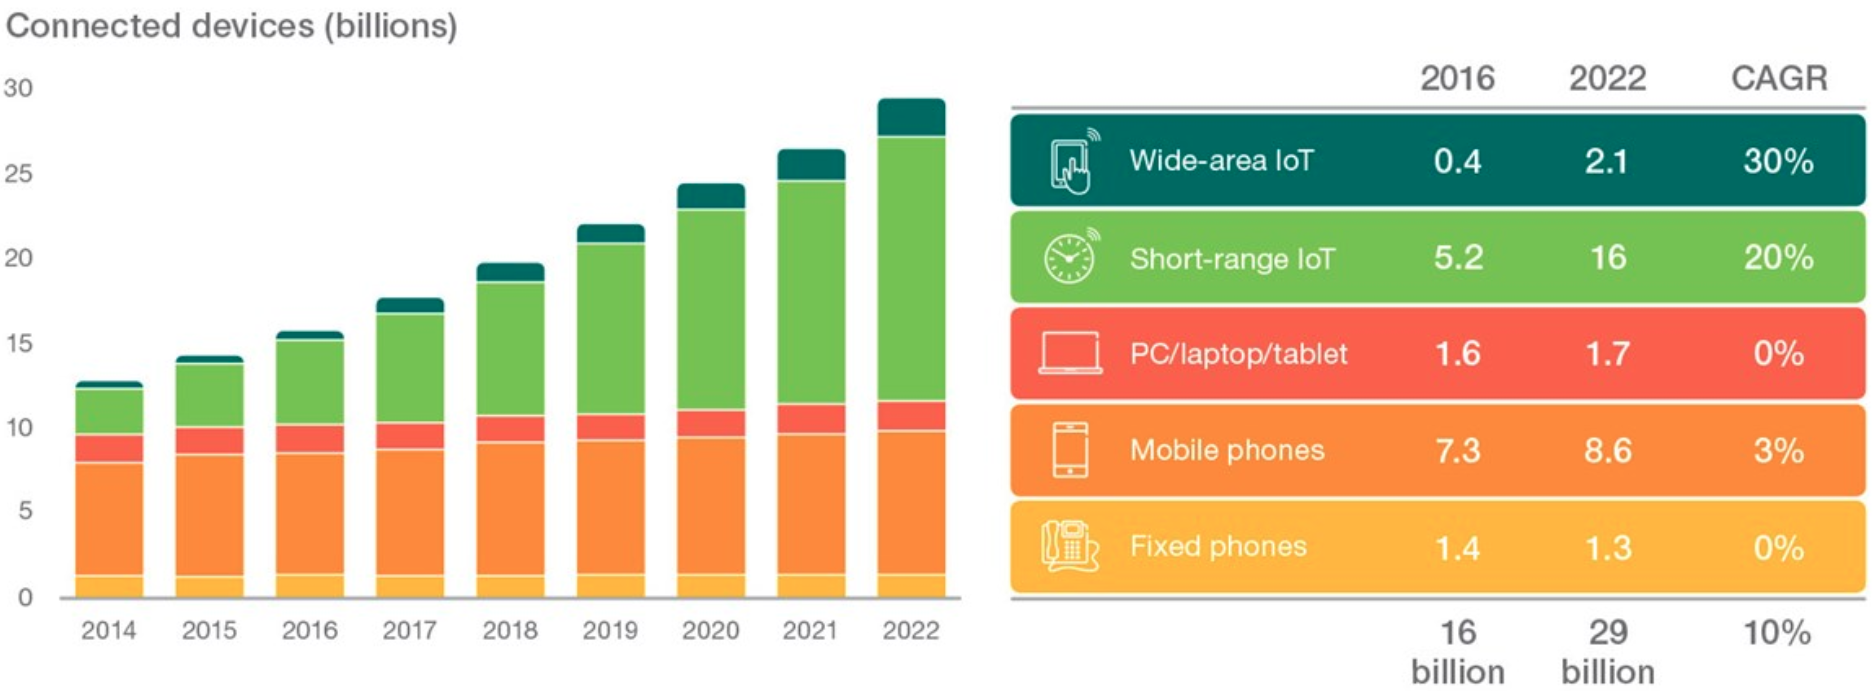
\includegraphics[width=.9\columnwidth]{devices1}
  \Figure{!htb}{1}{devices}{IoT devices \cite{perera_mosden_2013}}
  % \Figure{!htb}{.7}{devices.jpg}{IoT devices \cite{perera_mosden_2013}}
\end{frame}

\subsection{IoT Applications}
\begin{frame}{Applications diversification}{Each application has its own communication requirements}
  \Columns{0.6}{0.4}{
    \begin{table}[h!]
    \scriptsize
      \begin{tabulary}{\textwidth}{L|C|C|C|C|C}
      Challenges/Applications & Grids       & EHealth   & Transport     & Cities       & \textbf{Building}  \\\hline
      Resources constraints   & \ko         & \ok       & \ko           & \mm          & \ko                \\\hline
      Mobility                & \ko         & \mm       & \ok           & \ok          & \ko                \\\hline
      \textbf{Heterogeneity}  & \mm         & \mm       & \mm           & \ok          & \ko                \\\hline
      Scalability             & \ok         & \mm       & \ok           & \ok          & \mm                \\\hline
      QoS constraints         & \mm         & \mm       & \ok           & \ok          & \ok                \\\hline
      Data management         & \mm         & \ko       & \ok           & \ok          & \mm                \\\hline
      Lack of Standardization & \mm         & \mm       & \mm           & \mm          & \ok                \\\hline
      Amount of attacks       & \ko         & \ko       & \ok           & \ok          & \ok                \\\hline
      Safety                  & \mm         & \ok       & \ok           & \mm          & \ok                 \\\hline
      \end{tabulary}
    \caption{\label{tab:iot_challenges} Main IoT challenges \cite{kouicem_internet_2018} \cite{venkatesan_design_2017}}
    \end{table}
  }{
    \Figure{!htb}{1}{application}{IoT Applications}
  }
\end{frame}


% Current bad state, statistics with the problem
% \subsection{Context}
\begin{frame}{IoT platforms}{IoT platforms is a chain of communication process}
  \Figure{!htb}{.8}{context}{IoT platform}
  \Figure{!htb}{.9}{iotChallenges}{IoT challenges}
\end{frame}


\begin{frame}{Applications diversification}{Requirements} 
\begin{table}[h!]
\scriptsize
  \begin{tabulary}{\columnwidth}{L|C|C|L}
  \textbf{Use Case}                      & \textbf{Packet rate}   & \textbf{Min success rate} & \textbf{Payload Size}            \\
  \                               & \textbf{[pkt/day]}    & \textbf{[Ps,min]}     & \textbf{[Byte]}              \\\hline
  \textbf{Wearables}                     & 10                     &        90                 & \multirow{5}{*}{10-20}   \\
  \textbf{Smoke Detectors}               & 2                      &        90                 &                         \\
  \textbf{Smart Grid}                    & 10                     &        90                 &                         \\
  \textbf{White Goods}                   & 3                      &        90                 &         \\
  \textbf{Waste Management}              & 24                     &        90                 &         \\\hline
  \textbf{VIP/Pet Tracking}              & 48                     &        90                 & \multirow{9}{*}{50}        \\
  \textbf{Smart Bicycle}                 & 192                    &        90                 &         \\
  \textbf{Animal Tracking}               & 100                    &        90                 &         \\
  \textbf{Environmental Monitoring}      & 5                      &        90                 &         \\
  \textbf{Asset Tracking}                & 100                    &        90                 &         \\
  \textbf{Smart Parking}                 & 60                     &        90                 &         \\
  \textbf{Alarms/Actuators}              & 5                      &        90                 &         \\
  \textbf{Home Automation}               & 5                      &        90                 &         \\
  \textbf{Machinery Control}             & 100                    &        90                 &         \\\hline
  \textbf{Water/Gas Metering}            & 8                      &        90                 & \multirow{9}{*}{100-200}        \\
  \textbf{Environmental Data Collection} & 24                     &        90                 &         \\
  \textbf{Medical Assisted Living}       & 8                      &        90                 &         \\
  \textbf{Micro-generation}              & 2                      &        90                 &         \\
  \textbf{Safety Monitoring}             & 2                      &        90                 &         \\
  \textbf{Propane Tank Monitoring}       & 2                      &        90                 &         \\
  \textbf{Stationary Monitoring}         & 4                      &        90                 &         \\
  \textbf{Urban Lighting}                & 5                      &        90                 &         \\
  \textbf{Vending Machines Payment}      & 100                    &        90                 &         \\\hline
  \textbf{Vending Machines General}      & 1                      &        90                 & 1K        \\
  \end{tabulary}
\caption{\label{tab:zzes}Application requirements for the use cases of interest \cite{feltrin_lorawan_2018} \cite{venkatesan_design_2017} \cite{rizzi_evaluation_2017}}
\end{table}
\end{frame}

\subsection{IoT Wireless Communications}
\begin{frame}{IoT wireless communication}{Wireless communication performance need to be evaluated to match applications requirements}
  % \Columns{0.4}{0.6}{
    \Figure{!htb}{.7}{new-LPWAN}{Short range, Cellular and Long range networks}
  % }{
    % \Figure{!htb}{1}{snr}{SNR \& RSSI}
    % \Figure{!htb}{1}{ToA}{Time on air}
  % }
\end{frame}



\subsubsection{LoRa}

\begin{frame}{Wireless communication}{Exp: LPWAN in a new technology that satisfy IoT applications requirements}
  \Columns{0.55}{0.45}{
    %\Figure{!htb}{1}{LPWAN}{Wireless communication diversity}
  }{
    \Figure{!htb}{1}{lora_stack}{LoRa and LoRaWan stack}
  }
\end{frame}

\begin{frame}{LoRa parameters selection}{How to select the optimal configuration}
  \Columns{.5}{.5}{
    \begin{itemize}
    \item Parameters
      \begin{itemize}
      \item \ac{BW}
      \item \ac{SF}
      \item \ac{CR}
      \item \ac{P^{tx}}
      \item \ac{PS}
      \item \ac{SNR} [-7.5,-20dBm]
      \end{itemize}
    \end{itemize}
  }{
    \begin{itemize}
    \item Metrics
      \begin{itemize}
      % \item \ac{$S_{rx}$}
      \item \ac{DR}
      \item \ac{AT}
      \item $\ac{PS}_{max}$
      \item \ac{RSSI} [-30,-120dBm]
      \end{itemize}
    \end{itemize}
  }
  \medskip
  \begin{table}[h!]
  % \scriptsize
    \begin{tabular}{l|m{1mm}l|l|l}
    \textbf{Setting} & \multicolumn{2}{l|}{\textbf{Values}} & \textbf{Rewards}     & \textbf{Costs}                      \\\hline
    \ac{BW}          & $7.8 $                               & \ding{224} $500 kHz$ & \ac{DR}                              & \ac{RSSI}, \blue{Range}              \\\hline
    \ac{SF}          & $2^{6}$                              & \ding{224} $2^{12}$  & \ac{RSSI}, \blue{Range}            & \ac{DR}, \ac{SNR}, $\ac{PS}_{max}$, \ac{P^{tx}}   \\\hline
    \ac{CR}          & $4/5$                                & \ding{224} $4/8$     & \ac{SNR}                             & $\ac{PS}_{max}$, \ac{P^{tx}}, \ac{AT}       \\\hline
    \ac{P^{tx}}      & $-4$                                 & \ding{224} $20 dBm$  & \ac{SNR}                             & \ac{P^{tx}}                      \\\hline
    \ac{PS}          & $59$                                 & \ding{224} $230 B$   & \ac{PS}                              & \ac{P^{tx}}, \ac{AT}                \\\hline
    \end{tabular}
  \caption{\label{tab:} LoRa parameters selection \cite{marco_cattani_experimental_2017}}
  \end{table}
\end{frame}

\begin{frame}{Multi criteria decision making}
\begin{table}[h]
%\scriptsize
  \begin{tabular}{l|l|l}
  \textbf{Layer} & \textbf{Maximize (Reward)} & \textbf{Minimize (Cost)}\\\hline
  Application    & \blue{Sec} security        & \ac{SC}                 \\\hline
  Network        & \blue{Range}               & \ac{Jit}                \\
  \              & \ac{PDR}                   & \ac{TC}                 \\
  \              & \ac{PS}                    & \ac{RTD}                \\
  \              & \ac{DR}                    & \ac{PER}                \\
  \              &                            & \ac{O_{time}}           \\
  \              &                            & \ac{O_{space}}          \\\hline
  Radio          & \ac{Mob}                   & \ac{BER}                \\
  \              & \ac{SR}                    & \ac{P^{tx}}             \\
  \              & \ac{BR}                    & \ac{CCI}                \\
  \              & \ac{SIR}                   & \ac{DC}                 \\
  \              & \ac{RSSI}                  & \ac{ToA}                \\
  \              & \ac{SINR}                  & \ac{PL}                 \\
  \              & \ac{SNR}                   &                         \\
  \end{tabular}
\caption{\label{tab:scheduling} Network selection inputs and classification of parameters \cite{bendaoud_network_2019} \cite{chowdhury_survey_2018}}
\end{table}
\end{frame}


% \begin{frame}{ToA: Time on air}{Physical layer \cite{eriksson_investigating_2017}}
% \begin{align}
% \textbf{\ac{ToA}}_{LoRa}=                                       & \frac{2^{S F}}{B W}\left((N P+4.25)+\left(S W+\max \left(\left\lceil\frac{8 PS-4 S F+28+16 C R C-20 I H}{4(S F-2 D E)}\right](C R+4), 0\right)\right)\right)\\
% \textbf{\ac{ToA}}_{GFSK}=                                       & \frac{8}{D R}(N P+S W+P L+2 C R C)
% \end{align}
% \textbf{Where:}
% \Itemize{
%   \item NP = 8, if LoRa . 5, if GFSK
%   \item SW = 8, if LoRa . 3, if GFSK

%   \item CRC = 0 if downlink packet.        1 if uplink packet
%   \item IH  = 0 if header.                 1 if no header present
%   \item DE  = 1 if data rate optimization. 0 if not
% }
% \Itemize{
%   \item \ac{PS} = PHY\_Payload bytes
%   \item \ac{SF} = 7, 8, 9, 10, 11, 12
%   \item \ac{BW} = 125kHz, 250kHz, where BW is the bandwidth  
%   \item \ac{CR} = Indicates the Coding Rate
% }
% \end{frame}

\begin{frame}{Multi criteria decision making}
$\ac{ToA}_{LoRa}                 = \frac{2^{S F}}{B W}\left((N P+4.25)+\left(S W+\max \left(\left\lceil\frac{8 PS-4 S F+28+16 C R C-20 I H}{4(S F-2 D E)}\right](C R+4), 0\right)\right)\right)$\\

\Columns{.5}{.5}{
  \begin{align}
%   R_{c[chips/s]}           =& BW                                     \\
% R_{S[symbols/s]}       =& \frac{R_{c}}{2^{SF}} = \frac{BW}{2^{SF}}                \\
% R_{m}=\ac{DR}_{\textbf{[bps]}}    =& SF.RS=\red{SF}*\frac{\green{BW}_{[Hz]}}{2^{\red{SF}}}*\yellow{CR}    \\
  \ac{ToA}_{\textbf{GFSK}}    = & \frac{8}{D R}(N P+S W+P L+2 C R C) \\
  \ac{Sen}_{\textbf{[dBm]}}   = & -174+10 \log _{10} \green{BW} + NF + SNR                                                      \\
  \ac{PL}_{\textbf{[B]}}      = & |RSSI|+SNR+P_{TX}+G_{RX}                                                               \\
  \ac{SNR}_{\textbf{[dB]}}    = & 20.log(\frac{S}{N})                                                                           \\
  \ac{RSSI}_{\textbf{[dBm]}}  = & Tx_{power}.\frac{Rayleigh_{power}}{PL}                                                        \\
  \ac{SINR}_{\textbf{[dBm]}}  = \\
  \ac{BR}_{ \textbf{[bps]}}   = & \red{SF} * \frac{\frac{4}{4+\yellow{CR}}}{\frac{2 \red{SF}}{\green{BW}}}                      \\
  \ac{BER}_{\textbf{[bps]}}   = & \frac{8}{15}.\frac{1}{16}.\sum{k=2}{16}{-1^{k}(\frac{16}{k})e^{20.SINR(\frac{1}{k}-1)}}       \\
  \ac{PER}_{\textbf{[pps]}}   = & 1-(1-BER)^{n_{bits}}                                                                          \\
  \end{align}
}{
  \ \ \textbf{Where:}
  \Itemize{
    \item NP = 8, if LoRa . 5, if GFSK
    \item SW = 8, if LoRa . 3, if GFSK

    \item CRC = 0 if downlink packet.        1 if uplink packet
    \item IH  = 0 if header.                 1 if no header present
    \item DE  = 1 if data rate optimization. 0 if not
  }
  \Itemize{
    \item \ac{PS} = PHY\_Payload bytes
    \item \ac{SF} = 7, 8, 9, 10, 11, 12
    \item \ac{BW} = bandwidth  
    \item \ac{CR} = Indicates the Coding Rate
  }  
}
\end{frame}


% \begin{frame}{Multi criteria decision making}
% \begin{align}
% \ac{MSE}=                     & \frac{1}{n} \sum_{i=1}^{n}\left(p_{i}-r_{i}\right)^{2}                                        \\
% \ac{RMSE}=                    & \sqrt{\frac{1}{n} \sum_{i=1}^{n}\left(p_{i}-r_{i}\right)^{2}}                                 \\
% \ac{MAE}=                     & \frac{1}{n} \sum_{i=1}^{n}\left|p_{i}-r_{i}\right|                                            \\
% Recall=                       & \frac{T P}{T P+F N}                                                                           \\
% Precision=                    & \frac{T P}{T P+F P}                                                                           \\
% F1_{-}Score=                  & \frac{2 \times \text { Precision } \times \text { Recall}}{\text { precision }+\text {recall}}\\
% \ac{TPR} =                    & \frac{T P}{T P+F N}                                                                           \\
% \ac{FPR} =                    & \frac{F P}{F P+T N}                                                                           \\
% \ac{ROC}=                     & (TPR,FPR)                                                                                     \\
% Novelty=                      & \sum_{i \in L} \frac{\log _{2} P_{i}}{n} \text { where } \quad P_{i}=\frac{n-r a n k_{i}}{n-1}\\
% Serendipity=                  & \frac{1}{n} \sum_{i \in n} \max \left(P_{\text {user}}-P_{U}, 0\right) \times r e l_{i}       \\
% diversity=                    & \frac{a}{c} \sum_{i=1}^{c} \frac{1}{n} \sum_{j=1}^{n} i_{j}                                   \\
% Coverage=                     & 100 \times \frac{u}{U}                                                                        \\
% Stability=                    & \frac{1}{P_{2}} \sum_{i \in P_{2}}\left|P_{2, i}-P_{1, i}\right|                              \\
% DCG=                          & r e l_{1}+\sum_{i=2}^{\text {pos}} \frac{r e l_{i}}{\log _{2} i}                              \\
% IDCG=                         & r e l_{1}+\sum_{i=2}^{|h|-1} \frac{r e l_{i}}{\log _{2} i}                                    \\
% \ac{NDCG}=                    & \frac{D C G}{I D C G}                                                                         \\
% \ac{PRR} =                    & (1-\ac{BER})^{L}                                                                              \\
% \end{align}
% \end{frame}


% \begin{frame}
% \printacronyms[include-classes=nomencl,name=]
% \ac{SINR}
% \ac{SIR}
% \ac{BR}
% \ac{DR}
% \ac{BW}
% \ac{BER}
% \ac{PER}
% \ac{PRR}
% \ac{PDR}
% \ac{SNR}
% \ac{PLR}
% \ac{RTT}
% \ac{Tx}
% \ac{PS}
% \ac{TC}
% \ac{DC}
% \ac{SR}
% \ac{SL}
% \ac{Jit}
% \ac{CCI}
% \ac{ToA}
% \ac{PL}
% \ac{Mob}
% \ac{Th}
% \ac{SC}
% \ac{Sen}
% \ac{RSSI} 
% \ac{O_{time}}
% \ac{O_{space}}
% \ac{PktL}
% \ac{RS}
% \end{frame}



% \begin{frame}{Multi criteria decision making}
% \begin{table}[h]
% %\scriptsize
%   \begin{tabular}{l|l|l}
%   \textbf{Layer}                      & \textbf{Maximize (Reward)}             & \textbf{Minimize (Cost)}        \\\hline
%   Application              & \blue{Sec} security                   & \ac{SC}                      \\\hline
%   % \                  & Ergonomic                &                  \\

%     Network                             & \blue{Range}                & \ac{Jit}                       \\
%     \                                   & \ac{PDR}                   & \ac{TC}                 \\
%     \                                   & \ac{PS}                 & \ac{RTD}              \\
%     \                                   & \ac{DR}                & \ac{PER}      \\
%     \                                   &                       & \ac{O_{time}}            \\
%   \                                   &                        & \ac{O_{space}}          \\\hline

%   Radio                    & \ac{Mob}                 & \ac{BER}      \\                       
%   \                      & \ac{SR}                 & \ac{P^{tx}}               \\
%   \                      & \ac{BR}                & \ac{CCI}              \\
%   \                  & \ac{Sen}                 & \ac{DC}              \\
%   \                  & \ac{RSSI}               & \ac{ToA}                \\
%   \                  & \ac{SINR}               & \ac{PL}              \\
%   \                  & \ac{SNR}                 &                   \\
%   \                  & \ac{SIR}                &                   \\
%   \end{tabular}
% \caption{\label{tab:scheduling} Network selection inputs and classification of parameters \cite{bendaoud_network_2019} \cite{chowdhury_survey_2018}}
% \end{table}
% \end{frame}



% \begin{frame}{Multi criteria decision making}
% \begin{align}
% \ac{MSE}=                     & \frac{1}{n} \sum_{i=1}^{n}\left(p_{i}-r_{i}\right)^{2}                                        \\
% \ac{RMSE}=                    & \sqrt{\frac{1}{n} \sum_{i=1}^{n}\left(p_{i}-r_{i}\right)^{2}}                                 \\
% \ac{MAE}=                     & \frac{1}{n} \sum_{i=1}^{n}\left|p_{i}-r_{i}\right|                                            \\
% Recall=                       & \frac{T P}{T P+F N}                                                                           \\
% Precision=                    & \frac{T P}{T P+F P}                                                                           \\
% F1_{-}Score=                  & \frac{2 \times \text { Precision } \times \text { Recall}}{\text { precision }+\text {recall}}\\
% \ac{TPR} =                    & \frac{T P}{T P+F N}                                                                           \\
% \ac{FPR} =                    & \frac{F P}{F P+T N}                                                                           \\
% \ac{ROC}=                     & (TPR,FPR)                                                                                     \\
% Novelty=                      & \sum_{i \in L} \frac{\log _{2} P_{i}}{n} \text { where } \quad P_{i}=\frac{n-r a n k_{i}}{n-1}\\
% Serendipity=                  & \frac{1}{n} \sum_{i \in n} \max \left(P_{\text {user}}-P_{U}, 0\right) \times r e l_{i}       \\
% diversity=                    & \frac{a}{c} \sum_{i=1}^{c} \frac{1}{n} \sum_{j=1}^{n} i_{j}                                   \\
% Coverage=                     & 100 \times \frac{u}{U}                                                                        \\
% Stability=                    & \frac{1}{P_{2}} \sum_{i \in P_{2}}\left|P_{2, i}-P_{1, i}\right|                              \\
% DCG=                          & r e l_{1}+\sum_{i=2}^{\text {pos}} \frac{r e l_{i}}{\log _{2} i}                              \\
% IDCG=                         & r e l_{1}+\sum_{i=2}^{|h|-1} \frac{r e l_{i}}{\log _{2} i}                                    \\
% \ac{NDCG}=                    & \frac{D C G}{I D C G}                                                                         \\
% \ac{PRR} =                    & (1-\ac{BER})^{L}                                                                              \\
% \end{align}
% \end{frame}




 \begin{frame}{LoRa Frame}{}
   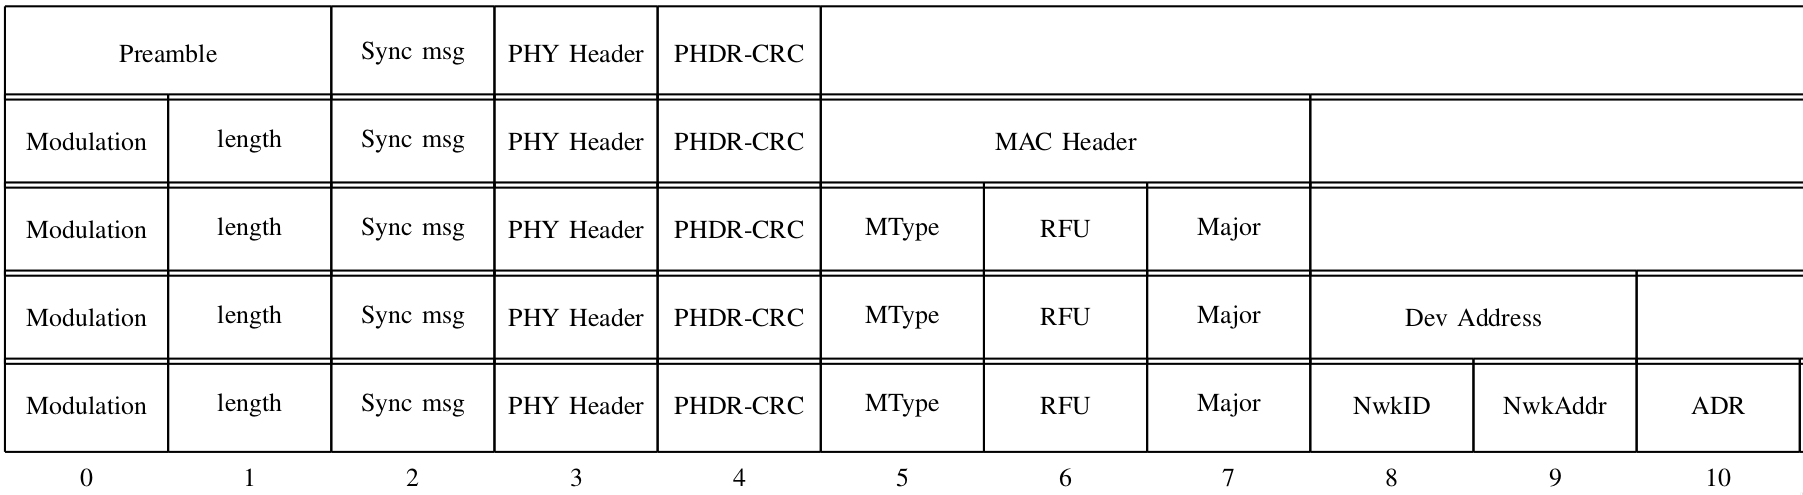
\includegraphics[width=1\columnwidth]{loraframe1}
   \bigskip
   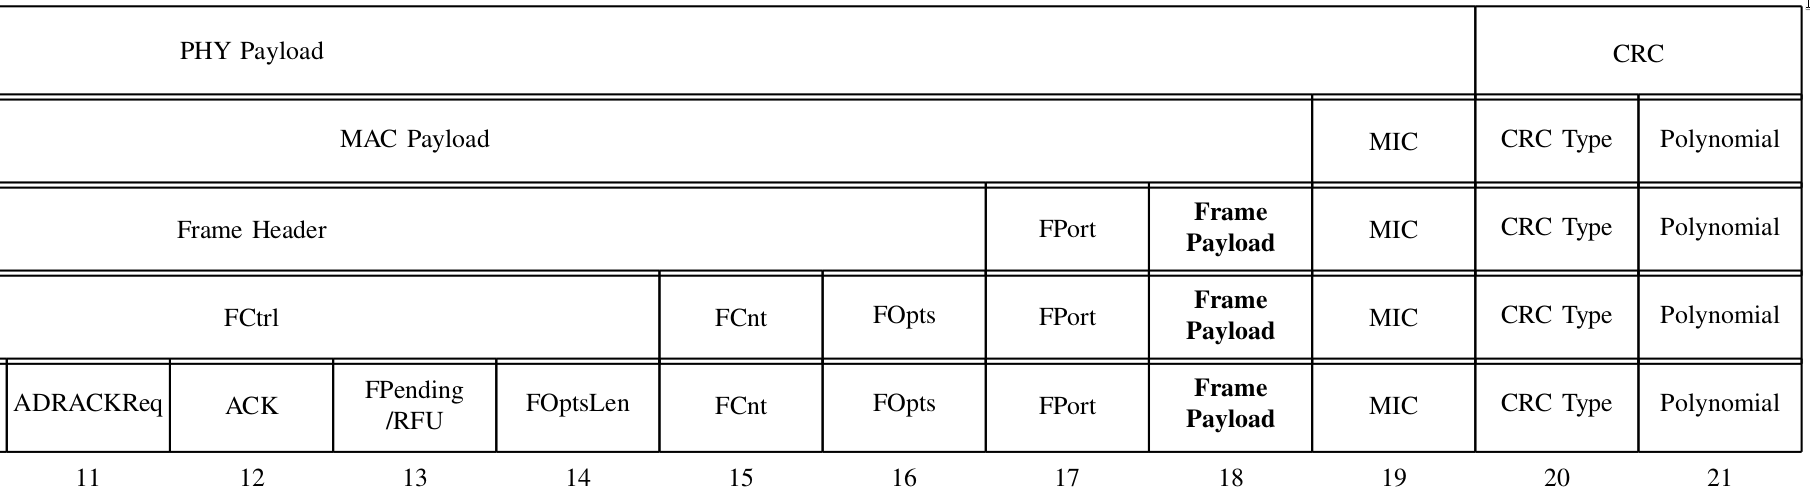
\includegraphics[width=1\columnwidth]{loraframe2}
 \end{frame}


 \begin{frame}{LoRa Frame}{}
\scriptsize
\begin{multicols}{2}
\Itemize{
  \item \textbf{Modulation :}
  \Itemize{
    \item Lora:  8 Symbols, 0x34 (Sync Word)
    \item FSK:  5 Bytes, 0xC194C1 (Sync Word)
  }
}
\Itemize{
  \item \textbf{Length :}
  \item \textbf{Sync msg :}
  \item \textbf{PHY Header :}  It contains:
  \Itemize{
    \item The Payload length (Bytes)
    \item \textbf{The Code rate}
    \item Optional 16bit CRC for payload 
  }
  \item \textbf{Phy Header :} CRC  It contains CRC of Physical Layer Header
  \item \textbf{MType :}  is the message type (uplink or a downlink)
  \Itemize{
    \item whether or not it is a confirmed message (reqst ack)
    \item 000   Join Request
    \item 001   Join Accept
    \item 010   Unconfirmed Data Up
    \item 011   Unconfirmed Data Down
    \item 100   Confirmed Data Up
    \item 101   Confirmed Data Down
    \item 110   RFU
    \item 111   Proprietary
  }
  \item \textbf{RFU :} Reserved for Future Use
  \item \textbf{Major :}  is the LoRaWAN version; currently, only a value of zero is valid
  \Itemize{
    \item 00   LoRaWAN R1
    \item 01-11   RFU
  }
  \item \textbf{NwkID :} the short address of the device (Network ID): 31th to 25th
  \item \textbf{NwkAddr :} the short address of the device (Network Address): 24th to 0th
  \item \textbf{ADR :}  Network server will change the data rate through appropriate MAC commands
  \Itemize{
    \item 1  To change the data rate
    \item 0  No change
  }
  \item \textbf{ADRACKReq :} (Adaptive Data Rate ACK Request): if network doesn't respont in 'ADR-ACK-DELAY' time, end-device switch to next lower data rate.
  \Itemize{
    \item 1  if (ADR-ACK-CNT) >= (ADR-ACK-Limit)
    \item 0  otherwise
  }
  \item \textbf{ACK :} (Message Acknowledgement): If end-device is the sender then gateway will send the ACK in next receive window  else if gateway is the sender then end-device will send the ACK in next transmission.
  \Itemize{
    \item 1  if confirmed data message
    \item 0  otherwise
  }
  \item \textbf{FPending$\downarrow$ /RFU $\uparrow$ :} (Only in downlink), if gateway has more data pending to be send then it asks end-device to open another receive window ASAP
  \Itemize{
    \item 1  to ask for more receive windows
    \item 0  otherwise
  }
  \item \textbf{FOptsLen :} is the length of the FOpts field in bytes   0000 to 1111 
  \item \textbf{FCnt :}  2 type of frame counters 
  \Itemize{
    \item FCntUp:  counter for uplink data frame, MAX-FCNT-GAP
    \item FCntDown:  counter for downlink data frame, MAX-FCNY-GAP
  }  
  \item \textbf{FOpts :} is used to piggyback MAC commands on a data message  
  \item \textbf{FPort :}  a multiplexing port field
  \Itemize{
    \item 0  the payload contains only MAC commands
     \item 1 to 223  Application Specific
     \item 224 \& 225  RFU
  }
    \item \textbf{FRMPayload :} (Frame Payload)  Encrypted (AES, 128 key length) Data                                 
  \item \textbf{MIC :}  is a cryptographic message integrity code
  \Itemize{
    \item computed over the fields MHDR, FHDR, FPort and the encrypted FRMPayload.
  }
  \item \textbf{CRC :} (only in uplink), 
  \Itemize{
    \item CCITT  $x^{16} + x^{12} + x^{5} + 1$
    \item IBM  $x^{16} + x^{15} + x^{5} + 1$
  }
}

\end{multicols}
 \end{frame}




%  \begin{frame}{Network selection problem}{Related work}
%    \Figure{h}{1}{slice2}{Network selection problem}
%  \end{frame}

%  \begin{frame}{Slice orchestration problem}{Related work}
%    \Figure{h}{1}{slice1}{Slice orchestration problem}
%  \end{frame}


% \begin{frame}{End-to-end Network slicing}{One size fits all problem: 1) Many configurations, 2) Diversity of service requirements}
%   \Figure{!htb}{.6}{slicing}{Key barriers in adopting IoT in the industry \cite{sciancalepore_storns_2019}}

%   % \bey{How to adapt the network to applications ?}
%   % \stamp{blue}{30}{6.2, 5}{How to adapt network configurations to applications ?}{90}

% \end{frame}

% \subsection*{Motivation}
% \begin{frame}{End-to-end Network slicing}{Exp: 4G/5G, Content provider (GAFA) want to be directly connected to users devices}
%   \Columns{0.5}{0.5}{
%     \Figure{!htb}{1}{slicing4}{Network slicing \cite{sciancalepore_storns_2019}}
%   }{
%     \FigureH{!htb}{1}{4G_slicing}{4G without network slicing}{5G_slicing}{5G with network slicing}{slicing3}{Network slicing concept \cite{sama_servicebased_2016}}
%   }
% \end{frame}

% \begin{frame}{Related work}{In the future, network administration function will disappear and will be replaced by a slice orchestrator}
%   % \tikz{\draw[red,thick,dashed] (2,2) circle (3cm);}
%   % \tikz{\draw[step=1cm,gray,very thin] (-1.9,-1.9) grid (5.9,5.9);}
%   \Figure{!htb}{.6}{slicing2}{Slice orchestrator \footcite{ksentini_toward_2017}}
%   % \bey{blue}{0}{6, 4}{\Huge Thank you !}
% \end{frame}


